\chapter{Results \& Summary}
\
\section{Wing Beat Cycle Motion Analysis}

\begin{figure}[H]
\centering
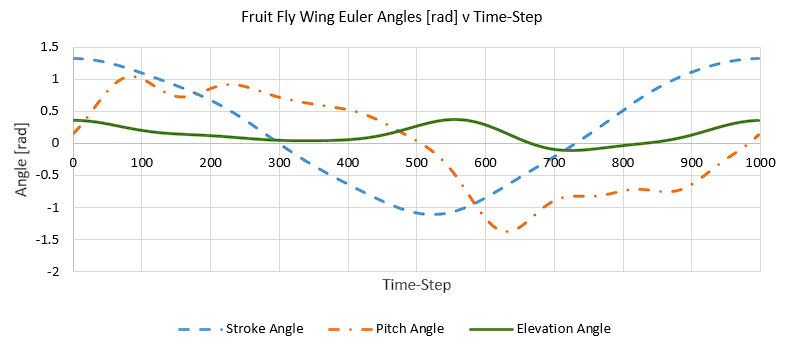
\includegraphics[width=\linewidth, ]{include/Euleranglesf.png}
\label{Euler Angles} 
\captionsetup{justification=centering}
\caption{Variation of fruit fly wing Euler angles across wing beat cycle}
\end{figure}

Before the discussion of results, initially, the discretization of the wing beat cycle and analysis of the kinematic wing beat motion are presented. By tracking the orientation of the wing according to the kinematics, different maneuvers carried out by the wing are tried to understand. The variation of the fruit fly wing Euler angles derived from the kinematics \cite{kinematics2,kinematics1}, measured with respect to the root coordinate system is plotted against time-step over a cycle in Fig 4.1.1.
\\
\\
The entire cycle of wing beat motion is discretized into 1000 time steps starting at T0 and ending at T1000. The frequency of wing beat considered for the study is 218 Hz \cite{kinematics2,kinematics1}. The time-step considered is $1/1000$ of the cycle time.
\\
\\
As we break down the wing beat motion into different time steps, the cycle is assumed to start from the extremum of the backward stroke at T0, and the forward stroke happens till the wing reaches the extremum of the forward stroke near T500. While near the extremum of the forward stroke, the pitch angle continuously changes from obtuse to acute. A similar change of pitch angle, this time acute to obtuse happens at the end of the backward stroke. The pitch angle changes at the extremum orienting the fruit fly wing at a positive angle of attack during both forward and backward strokes.
\\

The elevation angle of the wing has its local maxima while reaching the extremities of strokes. Also, the peculiar variation of the three angles during the extremities collectively depicts the flipping maneuver carried out by the fruit fly wing.

\section{Aerodynamic Characteristics of Fruit Fly Wing Beat Motion}

\begin{figure} [H]
\centering
\begin{tabular}{cccc}
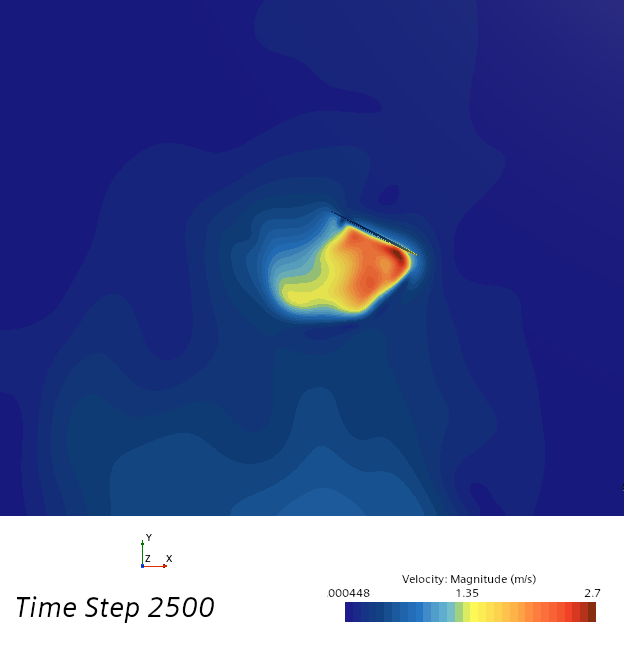
\includegraphics[width=0.4\textwidth]{include/2500ph.png} &
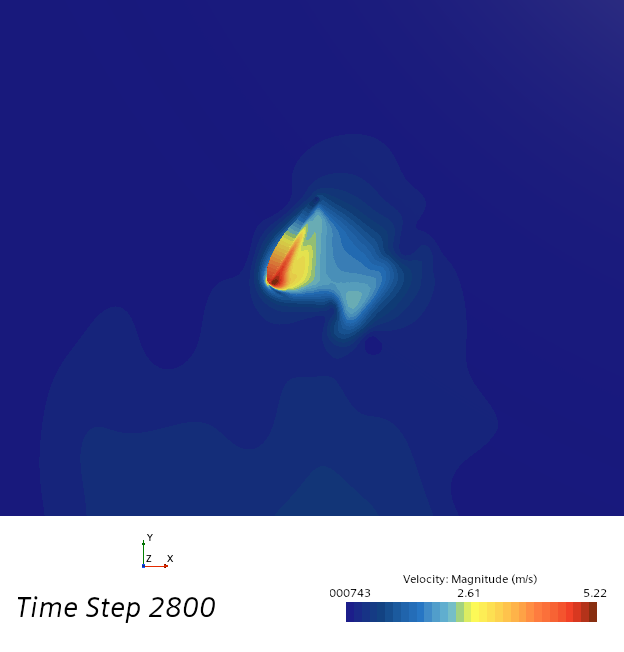
\includegraphics[width=0.4\textwidth]{include/2800ph.png} \\
\textbf{(a)}  & \textbf{(b)}\\[6pt]
\end{tabular}
\begin{tabular}{cccc}
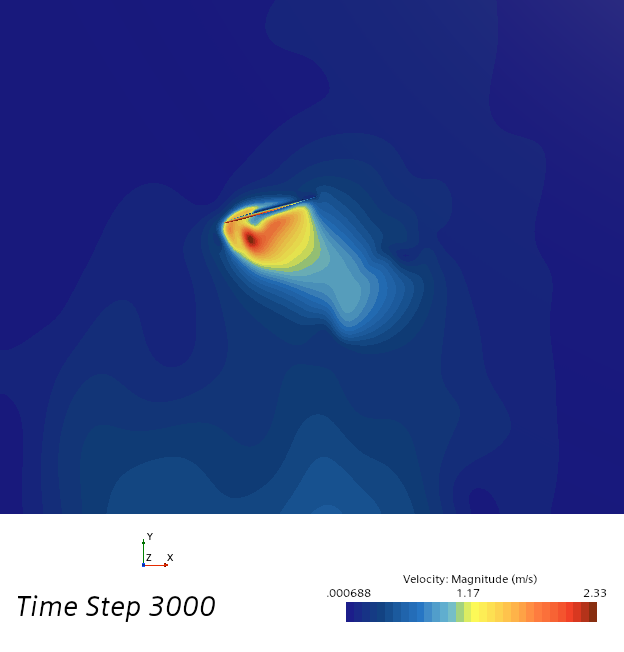
\includegraphics[width=0.4\textwidth]{include/3000ph.png} &
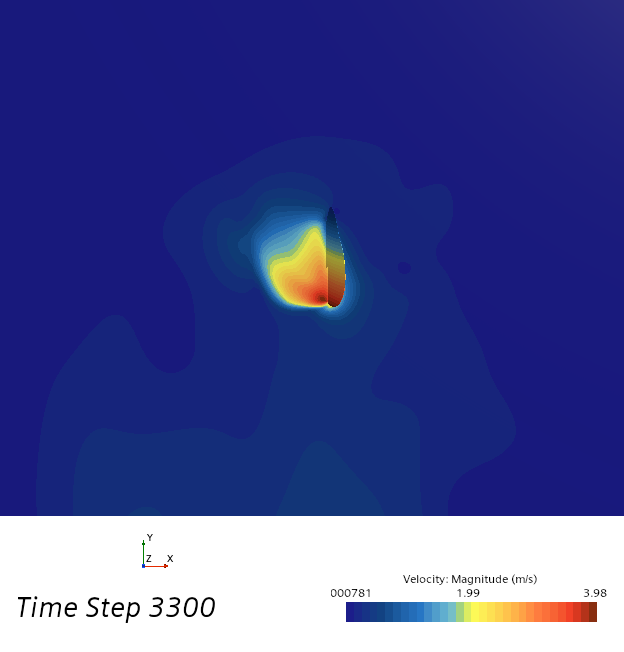
\includegraphics[width=0.4\textwidth]{include/3300ph.png} \\
\textbf{(c)}  & \textbf{(d)}  \\[6pt]
\end{tabular}
\captionsetup{justification=centering}
\caption{ \textbf{(a)} Extremum of backward stroke
\textbf{(b)} Intermediate position of forward stroke
\textbf{(c)} Extremum of forward stroke
\textbf{(d)} Intermediate position of backward stroke}
\label{fig: Velocity contour plots}
\end{figure}

The aerodynamic characteristics of the fruit fly wing motion obtained from CFD simulation are presented and discussed in this section. Eight wing beat cycles were simulated using CFD, and the results recorded for cycles 4 to 7 are used for interpretation. Since we are interested in the characteristics of the stabilized hovering motion of the fruit fly, the initial cycles are skipped. While observing the velocity field from CFD over different cycles, the flow field seemed to stabilize after 2 cycles. 
\\

Velocity contour of the flow field, variation of lift and drag over the wing beat cycle, pitching moment, and stroke moments are recorded for the specified cycles. The velocity contour taken on the z-plane at the mid-chord position of the wing recorded for different instances along the wing beat cycle is shown in Fig 4.2.1. 

\subsection{Lift \& Drag Characteristics}

\begin{figure}[H]
\centering
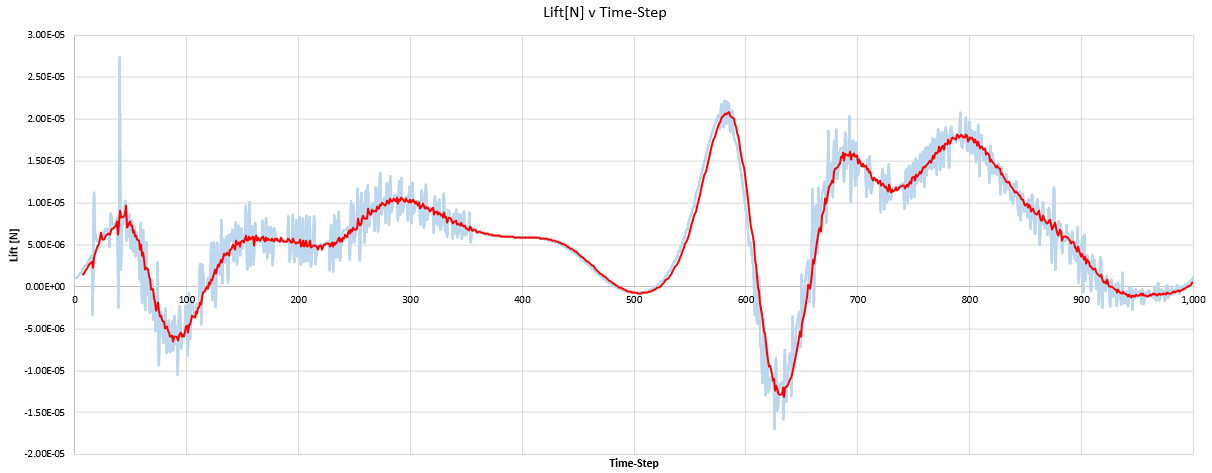
\includegraphics[width=\linewidth, ]{include/Liftplotf.png}
\label{Liftplot} 
\captionsetup{justification=centering}
\caption{Lift profile over wing beat cycle}
\end{figure}

The variation of lift generated by the wing over the wing beat cycle is plotted in Fig 4.2.2. The calculation of lift is made with respect to the stationary laboratory coordinate system. A moving average is used to smoothen the profile and an average is considered. The maximum of the lift profile is observed to be near T600. This region corresponds to the extremum of the forward stroke and is characterized by the pitch angle reversal. The fruit fly wing flips to orient itself at a positive angle of attack in preparation for the backward stroke. The eddies created by this complex motion as well as the low pressure created by the tail flow might have resulted in this peak lift. When we take the average lift over the entire cycle, a positive lift with a magnitude equal to 5.76   $\mu N$ per wing is observed. The mass of fruit-fly is considered to be equal to 1.2 $mg$ \cite{weight} and the lift produced corresponds to a lift-to-weight ratio approximately equal to 1. Considering the hovering motion of the fruit fly, the calculated lift-to-weight ratio being equal to one suggests reasonable adherence between simulated aerodynamic characteristics and reality.

\begin{figure}[H]
\centering
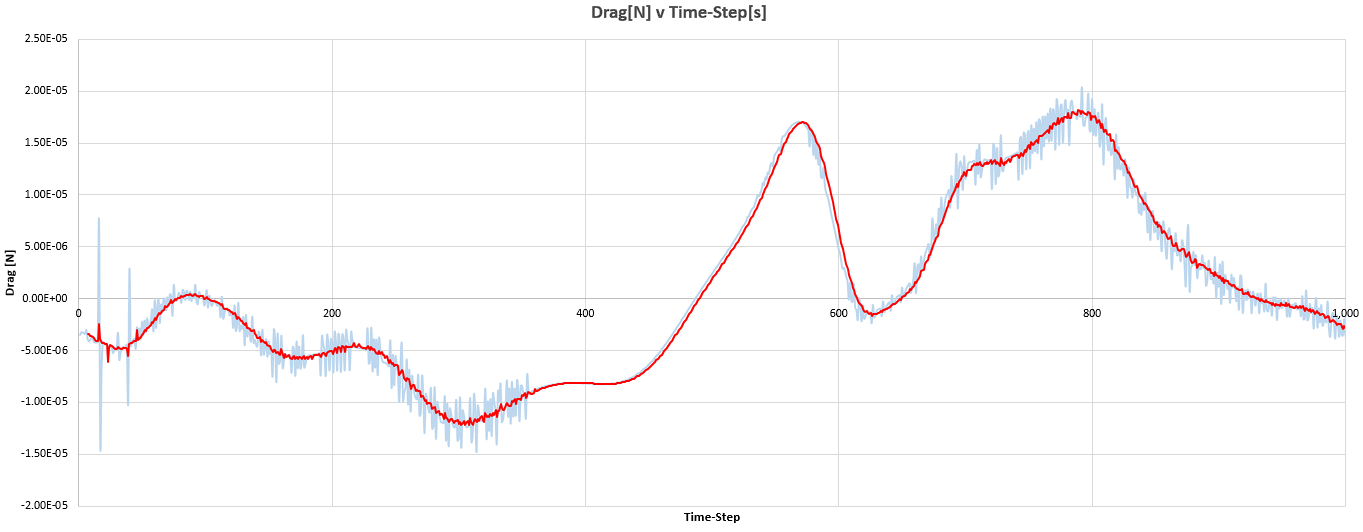
\includegraphics[width=\linewidth, ]{include/Dragplotf.png}
\label{Drag plot} 
\captionsetup{justification=centering}
\caption{Drag profile over wing beat cycle}
\end{figure}

The drag profile plotted for the wing beat cycle is shown in Fig 4.4. Similar to lift calculation the drag over the wing is measured with reference to the laboratory coordinate system. During the pitch reversal, the wing orient itself vertically at some point. This corresponds to the maximum drag point. The relative velocity of the backward stroke is higher compared to the forward stroke. This can result in a relatively high lift-induced drag. The similarity in lift and drag profile indicates this. The average drag measured over an entire cycle is 0.8 $\mu N$. The observed drag over the entire cycle is minimal. 

\subsection{Pitching Moment \& Stroke Moment Characteristics}

In this section, the pitching moment and stroke moment characteristics of the wing are studied. By evaluating the different moments exerted by the aerodynamic forces over the wing, the requirement for active involvement of fruit fly wing muscles is investigated.
\\
\\

\begin{figure}[H]
\centering
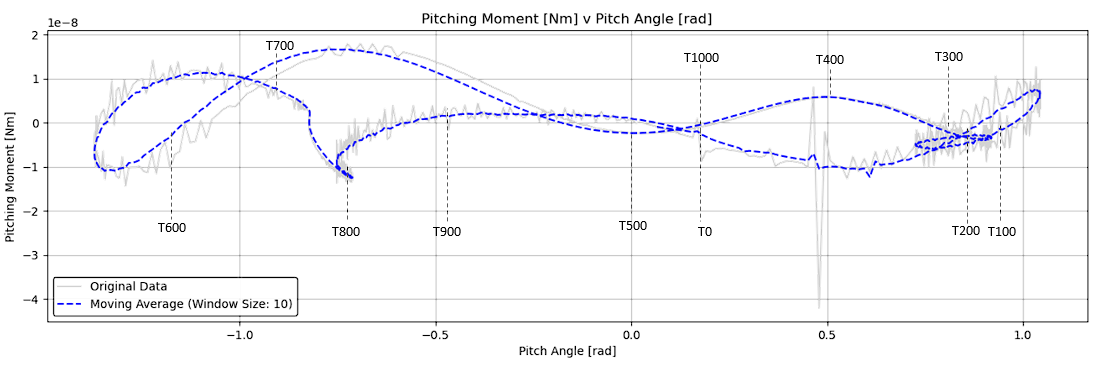
\includegraphics[width=0.95\linewidth, ]{include/pitchingmomentplotf.png}
\label{PMPlot} 
\captionsetup{justification=centering}
\caption{Pitching moment with respect to pitch angle variation over cycle}
\end{figure}
The pitching moment evaluated with respect to the wing root coordinate system is plotted against the pitch angle in Fig 4.5.

The absolute area inscribed by the pitching moment hysteresis loop is depicted in Fig 4.6. The magnitude of the absolute area inscribed is -2.56 $nJ$. The observed overall cycle hysteresis is negative which indicates insignificant energy expenditure over the complete cycle. Even though hysteresis over the complete cycle is near zero, we can observe the curve to self-intersect at different instances along the forward and backward strokes. 
\begin{figure}[H]
\centering
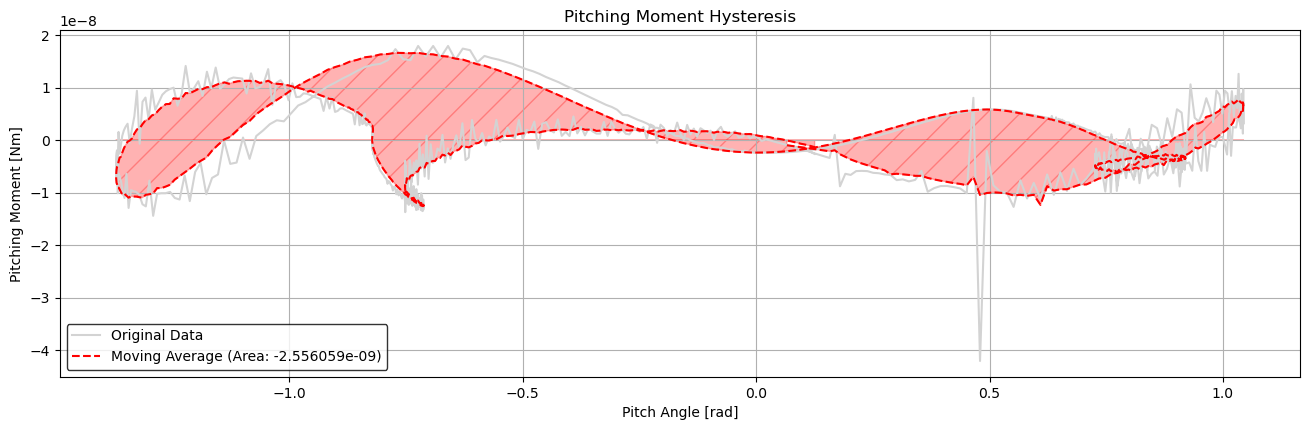
\includegraphics[width=0.95\linewidth, ]{include/PMHplot.png}
\label{PMhysteresisPlot} 
\captionsetup{justification=centering}
\caption{Pitching moment hysteresis over a cycle}
\end{figure}

The dissipators like muscle tissue in insects are characterised by a continuous hysteresis loop \cite{nguyen2020rheological}. The self-intersecting curves indicate the involvement of muscles in the pitch motion. Also, the reversal of the loop observed near T600 can be a scenario of dynamic stall and vortex shedding since the wing is in near vertical orientation and beyond normal stall angle \cite{dynamicstall1}. The dynamic stall seems to continue till T800 where the sharp region is observed. Beyond this point, a relatively stable variation of pitching moment is observed. This indicates the flow getting re-attached to the wing. As we observe the instances after the extremum of a backward stroke at T100, a rather complex profile is observed. Between T100 and T300 the curve intersects itself twice. The variation of pitch angle in this region is rapid and this can also be a case of flow separation and dynamic stall. The regions of significant hysteresis are in common characterised by the pitch angle reversal. As also seen in the pitch angle variation in Fig 4.1, the pitch angle seems to be almost steady in between the stroke extremes and with a peculiar waviness.

When comparing the pitching moment profile with lift data, we can observe that the local maxima of lift seem to match the regions of pitching moment reversal. This is indicative that the vortex shedding made by the rapid variation in pitch angle is aiding the lift generation by the wing. 
\begin{figure}[H]
\centering
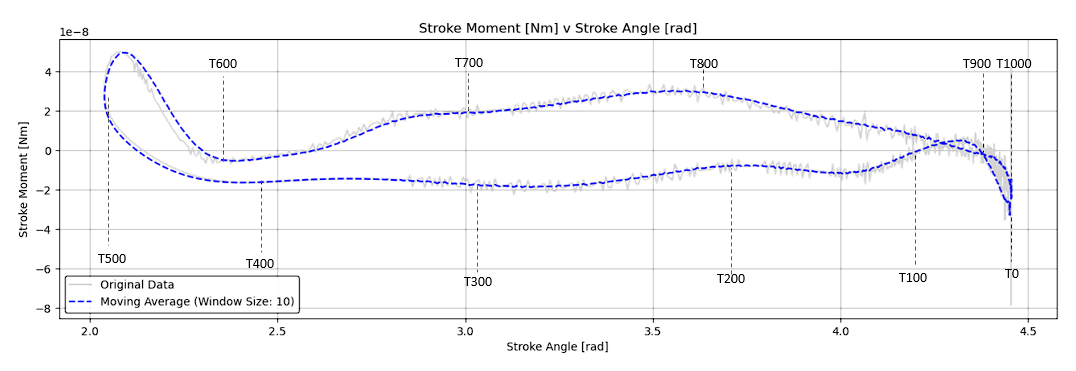
\includegraphics[width=0.95\linewidth, ]{include/smplotf.png}
\label{PMPlot} 
\captionsetup{justification=centering}
\caption{Stroke moment with respect to stroke angle variation over cycle}
\end{figure}
The stroke moment evaluated with respect to the wing root coordinate system is plotted against the stroke angle in Fig 4.7. The stroke moment hysteresis over the cycle is shown in Fig 4.8. The observed variation is similar to those found in literature \cite{Pons_2023}.

\begin{figure}[H]
\centering
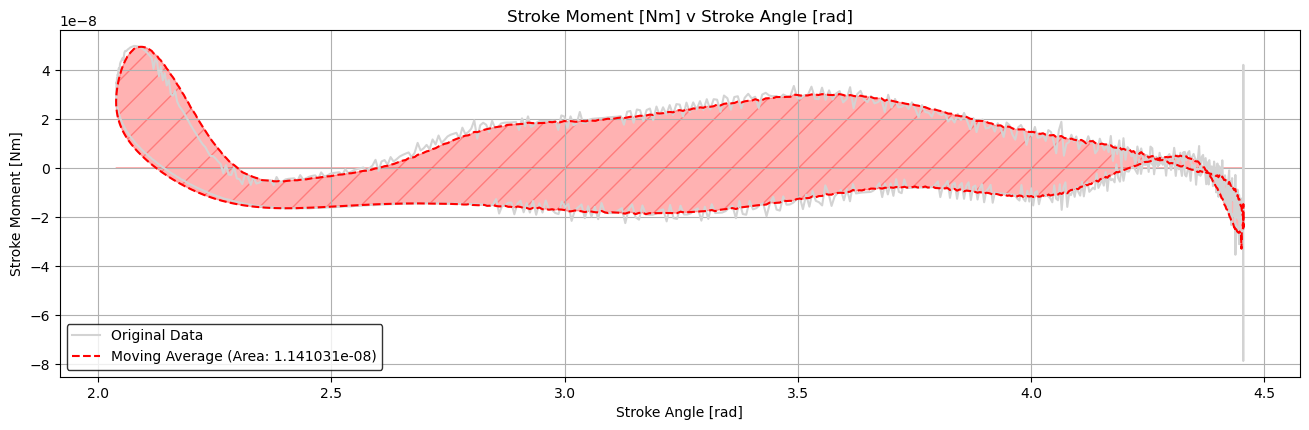
\includegraphics[width=0.95\linewidth, ]{include/SMHplot.png}
\label{SMHPlot} 
\captionsetup{justification=centering}
\caption{Stroke moment hysteresis over a cycle}
\end{figure}

While analyzing the stroke moment variation, we can notice significant variations near the extremes of strokes. At T0 where the backward stroke ends, the curve is intersecting and the moment value is undergoing a sudden drop. This indicates dynamic stall and vortex shedding. Between T500 and T600 also there exists a noticeable increase in stroke moment. Unlike the variation at T0, the variation at the end of the forward stroke is less rapid and relatively smooth. 
\\
\\
The absolute area of the hysteresis loop is positive and this indicates that work is done by the wing during the stroke motion. The magnitude of the hysteresis loop area is 11.4 $nJ$.

\section{Summary}

The complex unsteady maneuver of the wing at the extremities of forward and backward strokes creates significant variations in pitching moment and stroke moment characteristics.
\\
\\
The stroke motion hysteresis underlines the active nature of stroke motion. Self-intersecting behavior of the pitching moment curve indicates active involvement of insect muscles during pitch reversal. Also, the nature of the variations in pitching moment and stroke moment indicate that the wing is subjected to dynamic stall during pitch reversal. Even though there is a noticeable variation in lift and drag at these positions, sufficient average lift is maintained by the wing. We observed an increase in elevation angle accompanying the pitch reversal. While this maneuver may aid the pitch reversal process, it might also compensate for the decrease in lift due to stall. Apart from the extremities of the cycle, pitch motion seems to be passive with minimal hysteresis involved. To summarize, even though hysteresis for the pitch motion adds up to a negative value, the pitch reversal process might be partially active either by contribution from a muscle or coupling from an active elevation motion. 
\\
\\
The approach presented in the study considered the fruit fly wing as a rigid body. A fully coupled CFD simulation involving non-linear flexible wing effects can be a future scope of this project. 

\bibliographystyle{plain}  % Choose your preferred style
\bibliography{include/mendeley}  % Replace with your actual .bib file name (without extension)
